\documentclass{report}
\usepackage{amsmath,amssymb,amsthm,textcomp,gensymb,nccmath}
\usepackage{mathtools}
\renewcommand{\qedsymbol}{$\blacksquare$}

\setlength{\topmargin}{0.5in}
\usepackage[margin=4cm]{geometry}
\usepackage{enumerate}

\usepackage{setspace}
\onehalfspacing
\usepackage{parskip}
\setlength{\parskip}{0.5em}
\usepackage[T1]{fontenc}
\usepackage{palatino}

% useful characters/operators
\newcommand{\R}{\mathbb{R}}
\newcommand{\C}{\mathbb{C}}
\newcommand{\Z}{\mathbb{Z}}
\newcommand{\Q}{\mathbb{Q}}
\newcommand{\N}{\mathbb{N}}
\newcommand{\matP}{\mathbb{P}}
\newcommand{\mats}{\mathbb{s}}
\newcommand{\matH}{\mathbb{H}}
\newcommand{\matT}{\mathbb{T}}
\newcommand{\st}{\ s.t.\ }
\newcommand{\ie}{\ i.e.\ }
\newcommand{\eg}{\ e.g.\ }
\def \diam {\operatorname{diam}}
\def \Hom {\operatorname{Hom}}
\def \id {\operatorname{id}}
\def \tr {\operatorname{tr}}
\def \rk {\operatorname{rk}}
\def \dist {\operatorname{dist}}
\def \intr {\operatorname{int}}
\def \sgn {\operatorname{sgn}}
\def \im {\operatorname{Im}}
\def \re {\operatorname{Re}}
\def \curl {\operatorname{curl}}
\def \divg {\operatorname{div}}
\def \GL {\operatorname{GL}}
\def \Aut {\operatorname{Aut}}
\def \per {\operatorname{per}}
\newcommand{\pdr}[2]{\dfrac{\partial #1}{\partial #2}}
\newcommand{\dr}[2]{\dfrac{\text{d} #1}{\text{d} #2}}
\newcommand{\df}{\text{d}}
\newcommand{\inner}[2]{\left\langle #1, #2\right\rangle}

% arrows and :=, =:
\makeatletter
\providecommand*{\twoheadrightarrowfill@}{%
  \arrowfill@\relbar\relbar\twoheadrightarrow
}
\providecommand*{\twoheadleftarrowfill@}{%
  \arrowfill@\twoheadleftarrow\relbar\relbar
}
\providecommand*{\xtwoheadrightarrow}[2][]{%
  \ext@arrow 0579\twoheadrightarrowfill@{#1}{#2}%
}
\providecommand*{\xtwoheadleftarrow}[2][]{%
  \ext@arrow 5097\twoheadleftarrowfill@{#1}{#2}%
}
\makeatother

\newcommand{\defeq}{\vcentcolon=}
\newcommand{\eqdef}{=\mathrel{\mathop:}}

% integral for measure theory
\newcommand{\lowerint}{\underline{\int_{\R^d}}}
\newcommand{\upperint}{\overline{\int_{\R^d}}}
\newcommand{\lint}[1]{\underline{\int_{\R^d}} #1 (x)dx}
\newcommand{\uint}[1]{\overline{\int_{\R^d}} #1 (x)dx}
\newcommand{\sint}[1]{\simp{\int_{\R^d} #1 (x)dx}}
\newcommand{\lesint}[1]{\int_{\R^d} #1 (x)dx}

% note taking
\newcommand{\fancyem}[1]{\underline{\textsc{#1}}}

% theorem style
\newtheorem{theorem}{Theorem}[section]
\newtheorem{corollary}{Corollary}[section]
\newtheorem{lemma}{Lemma}[section]
\newtheorem{conjecture}{Conjecture}[section]
\newtheorem{proposition}{Proposition}[section]

\theoremstyle{definition}
\newtheorem{definition}{Definition}[section]
\newtheorem{example}{Example}[section]
\theoremstyle{remark}
\newtheorem*{remark}{Remark}

% for clearer reference
\usepackage{hyperref}
\newcommand{\corollaryautorefname}{Corollary}
\newcommand{\lemmaautorefname}{Lemma}
\newcommand{\definitionautorefname}{Definition}
\newcommand{\exampleautorefname}{Example}
\newcommand{\conjectureautorefname}{Conjecture}
\renewcommand{\subsectionautorefname}{Section}

% other styling
\usepackage{fancyvrb, fancyhdr}
\usepackage{tikz}
\PassOptionsToPackage{usenames, x11names}{xcolor}
\usepackage{tcolorbox}
\selectcolormodel{cmy}

\pagestyle{fancy}
\fancyhead[LO,L]{\leftmark}
\fancyhead[RO,R]{Yiwei Fu}
% \fancyhead[C]{MATH 566}
\fancyfoot[CO,C]{\thepage}
\renewcommand{\sectionmark}[1]{\markboth{#1}{#1}}

\numberwithin{equation}{section}

\newcommand{\fnl}{\parbox[t]{0\linewidth}{}}

% combinatorics special
\usepackage{pgfopts}
\usepackage{ytableau}

\begin{document}
\title{Notes for Math 566 -- Algebraic Combinatorics}
\author{Yiwei Fu}
\date{WN 2022}
\maketitle


\tableofcontents
Office hours: Tu, Fr 1:00 - 2:20 pm, 4868 East Hall.

\clearpage
\pagenumbering{arabic}

\chapter{Graph and Trees}
\section{Linear Algebra Preliminaries}
Let $M$ be a $p \times p$ matrix with entries in $\C$. The eigenvalues $\lambda_1, \lambda_2, \ldots, \lambda_p$ are defined by
\[
\det(t\id - M) = \prod_{i=1}^p (t - \lambda_i).
\]
Taking coefficients of $t^{p-1}$ on both sides we obtain
\begin{equation}\label{eq:trace}
\tr{M} = \sum_k \lambda_k.
\end{equation}


\begin{lemma}
Let $f(t) \in \C[t].$ Then $f(M)$ have eigenvalues $f(\lambda_1), \ldots, f(\lambda_p).$\end{lemma}
\begin{proof}
If $M$ is diagonalizable, then the statement is clear: $f(M)$ has the same eigenvectors as $M$, with eigenvalues $f(\lambda_k)$. Then use a continuity argument. (Diagonalizable matrices are dense.) Alternative proof: use Jordan’s normal form.
\end{proof}

Combining \eqref{eq:trace} with the lemma, we have
\begin{equation}\label{eq2}
\tr M^{\ell} = \sum_{k} \lambda_k^\ell.
\end{equation} 

\fancyem{Problem:} [A solution is given in Stanley’s textbook.] Let $\alpha_1, \ldots, \alpha_r$ and $\beta_1, \ldots, \beta_r$ be nonzero complex numbers such that for \emph{all} positive integer $\ell$ we have
\[
\alpha_1^\ell + \ldots + \alpha_r^\ell = \beta_1^\ell + \ldots + \beta_r^\ell.
\]
Show that this implies that $r=s$, and that $\alpha$'s are a permutation of $\beta$'s.

In the majority of forthcoming applications, $M$ is symmetric and real. Then it is diagonalizable, with real eigenvalues $\lambda_1, \ldots, \lambda_p$.

\section{Counting Walk}
Let $G$ be a graph on the vertex set $\{1, \ldots, p\}$. (We allow loops and multiple edges.) Let $M = A(G)$ be its adjacency matrix.

\fancyem{Observation} The number of walks of length $\ell$ from $i$ to $j$ is equal to $(M^\ell)_{ij}$.

In general, counting walks requires knowing the matrix $M$ (equivalently, knowing both the eigenvalues $\lambda_k$ and the corresponding eigenvectors). On the other hand, some enumerative information can be extracted from the eigenvalues alone:

\begin{proposition}
The number of marked closed walks of length $\ell$ is equal to $\sum_{k=1}^p \lambda^\ell_k$.
\end{proposition}
Here "marked" means that the starting location is fixed, as is a particular instance
of passing through it, in case we do it several times.

\begin{proof}
By the last observation, the number of marked closed walks of length $\ell$ is equal to $\tr M^\ell$, which equals to $\sum_{k=1}^p \lambda^\ell_k$ by \eqref{eq2}.
\end{proof}

\begin{example}
Let $G = K_p$, the complete graph on $p$ vertices. Let $J$ denote the $p \times p$ matrix all of whose entries are $1$. Let $I$ denote the $p \times p$ identity matrix. Then $A(G) = J - I$. Obviously $\rk J = 1$ and $\tr J = p$. Hence the eigenvalues of $J$ are $0, \ldots, 0, p$, and the eigenvalues of $A(G) = J - I$ are $-1, \ldots, -1, p-1$.
\end{example}

\begin{corollary}
There are $(p-1)^\ell + (-1)^\ell(p-1)$ marked closed walks of length $\ell$ in $K_p$.
\end{corollary}

\fancyem{Note} This is the number of $(\ell+1)$-letter words in a $p$-letter alphabet in which no two consecutive letters are identical, and which begin and end by the same letter.



\fancyem{Problem} Show that the number of walks of length $\ell$ between two distinct vertices in $K_p$ differs by $1$ from the number of closed walks of length $\ell$ starting at a given vertex.

\section{Eigenvalues of Adjacency Matrices}
\fancyem{Recall}
\[\# \text{ of marked closed walks of length } \ell = \sum_{i=1}^p \lambda_i^\ell.\]
It can be used backwards: using counted walks to compute eigenvalues.

\begin{example}
Let $G = K_{n, m}$ a complete bipartite graph. 
\[\# \text{ of marked closed works of length } \ell = \begin{cases}
0 & \ell = 2k + 1 \\
2n^{\ell/2}m^{\ell/2} & \ell = 2k
\end{cases} = (\sqrt{nm})^\ell + (-\sqrt{nm})^{\ell}
\]
$\xRightarrow[]{\text{Problem}}$ eigenvalues are $\sqrt{nm}, -\sqrt{nm}, 0, \ldots, 0.$
\end{example}

\fancyem{Problem} Prove that, for $G$ connected, the $\diam(G) < \# \text{ of distinct eigenvalues}.$

\begin{example}
$K_p = 1 < 2, K_{n, m} = 2 < 3.$
\end{example}

\section{Inequalities for the Maximal Eigenvalue}
\begin{definition}
Suppose $G$ a graph with vertices $= \{1, \ldots, p\}.$ Let
\[\lambda_{\max} \defeq \max_i|\lambda_i| = \max \lambda_i.\]
\end{definition}

\begin{proposition}
\[\lambda_{\max} \leq \max \deg(G)\]
\end{proposition}
\begin{proof}
For any vector $X = (x_k) \in \C^p$,
\[
\max_j|(A(G)X)_j| \leq \max \deg(G) \cdot \max_k|X_k|
\]
Now suppose $X$ is an eigenvector of $A(G)$ with eigenvalue $\lambda$. Then
\[
\max_j|(A(G)X)_j| = |\lambda| \max_k|X_k| \leq \max \deg(G) \cdot \max_k|X_k| \implies |\lambda| \leq \max \deg(G)
\]
This holds for all eigenvalue $\lambda_i$, which proves our proposition.
\end{proof}
\fancyem{Alternate proof:} by counting closed walks ($\leq \sum \max\deg(G)^\ell$.)

\fancyem{Problem} Prove that $\lambda_{\max} \geq $ average degrees of the vertices of $G$.\\
\fancyem{Hint} for symmetric real matrix $M$ we have $\lambda_{\max} = \max_{|x| = 1} x^{T}Mx.$

\begin{corollary} 
$\#$ of closed walk of length $\ell$ grows exponentially in $\ell$ with a rate $\geq$ average degree.
\end{corollary}


\section{Eigenvalue of Block Anti-diagonal Matrices}
\[M = \begin{bmatrix}
0 & B \\ B^{T} & 0
\end{bmatrix} \in \R_{n + m}\]

\begin{lemma}
The non-zero eigenvalues (called "singular values" of $B$) of $M$ are $\pm \sqrt{\mu_i}$ where $\mu_i$ are nonzero eigenvalues of $B^TB$ with multiplicities.
\end{lemma}
Note that $B^TB$ is positive definite.
\begin{proof} 
Let $F_X(t) = \det(t\id_p - X).$
\[
\begin{bmatrix}
t\id_n & -B \\
-B^T & t\id_m
\end{bmatrix}
\begin{bmatrix}
\id_n & B \\
0 & t\id_m
\end{bmatrix} = \begin{bmatrix}
t\id_n & 0 \\
-B & -B^TB + t^2\id_m
\end{bmatrix}
\]
\[
F_M(t) \cdot t^m = t^n F_{B^TB}(t^2)
\]
and the claim follows
\end{proof}

So now we are equipped to compute the eigenvalue of bipartite graphs.
\begin{example}
Suppose $G = K_{n, m}, B^TB$ is $m \times m$ matrix with all entries being $n$.
So the eigenvalues of $B^TB = nm, 0, 0, \ldots.$ So eigenvalues of $A(G)$ is $\sqrt{mn}, -\sqrt{mn}, 0, 0, \ldots$
\end{example}

\fancyem{Problem} Let $G$ to be the graph obtained by removing $n$ disjoint edges from $K_{n, n}.$ Find the eigenvalue of $G$.

\begin{example}
Let $G$ be a $2n$-cycle. $M_{2n} = A(G) = \begin{bmatrix}
0 & B \\ B^T & 0
\end{bmatrix}.$
The $B^TB = 2I_n + M_n$ for an appropriate labeling.

So if the eigenvalue of $n$-cycle are $\lambda_1, \ldots, \lambda_n.$ Then the eigenvalues of $2n$-cycles are $\pm\sqrt{\lambda_i + 2}.$
\end{example}

\section{Eigenvalues of Circulant Matrices}
\begin{definition}
A circulant matrix is of the form
\[
M = \begin{bmatrix}
s_0 & s_1 & s_2 & \ldots & s_{p-1} \\
s_{p-1} & s_0 & s_1 & \ldots & s_{p-2} \\
\vdots \\
s_1 & s_2 & s_3 & \ldots & s_0
\end{bmatrix}.
\]
\end{definition}

\begin{lemma}\label{le:circulant}
$M$ has eigenvalues \[\lambda_k = \sum_{j=0}^{p-1} s_je^{\tfrac{2\pi i}{p}jk}, k = 0, 1,\ldots, p-1.\]
\end{lemma}
Notice that
\[\lambda_k = \sum_{j=0}^{p-1} s_j e^{\tfrac{2\pi i}{p}jk} = s\left(e^{\tfrac{2\pi i}{p}k}\right) \quad \text{$p$-th root of unity}.\]
where \[s(x) = \sum_{j=0}^{p-1} s_j x^j.\]

\begin{proof}
Let \[
T = \begin{bmatrix}
0 & 1 & 0 & \ldots & 0 \\
0 & 0 & 1 & \ldots & 0 \\
\vdots \\
1 & 0 & 0 & \ldots & 0
\end{bmatrix}
\]
We have that the eigenvalues of $T$ and $p$-th roots of unity and characteristic polynomial is $t^p - 1.$

Key observation:
$M = s(T).$
\end{proof}

\begin{definition}
A graph $G$ is circulant if $A(G)$ is circulant, for some choice of vertex labeling.
\end{definition}
\begin{corollary}
The eigenvalue of $p$-cycle are 
\[2\cos\left(\frac{2\pi k}{p}\right), k = 0, 1, \ldots, p - 1.\]
\end{corollary}

\begin{proof}
By \autoref{le:circulant}, we have that
\[\lambda_k = e^{\tfrac{2 \pi i}{p}k} + e^{\tfrac{2 \pi i}{p}(p - 1)k} = e^{\tfrac{2 \pi ik}{p}} + e^{-\tfrac{2 \pi i k}{p}} = 2\cos\left(\frac{2\pi k}{p}\right). \qedhere\]
\end{proof}
\begin{remark}
This formula is consistent with the formula linking the eigenvalues of a $2n$-cycle and an $n$-cycle: if $2\cos\alpha = \lambda,$ then $2\cos\mfrac{\alpha}{2} = \pm\sqrt{2 + \lambda}.$
\end{remark}
\fancyem{Problem} Find the eigenvalues of the graph obtains by removing $n$ disjoint edges from $K_{2n}.$

\section{Eigenvalues of Cartesian Products}
\begin{definition}
Suppose $G, H$ are graphs with no loops. Define graph $G \times H$ where \[V(G \times H) = \{(g, h) : g \in V(G), h \in V(H)\},\]
and we have two kinds of edges:
\begin{itemize}
\item $(g, h) - (g', h)$ for $g - g'$
\item $(g, h) - (g, h')$ for $h - h'$
\end{itemize}
\end{definition}
\begin{example}
\begin{enumerate}
\item Grid graph = path $\times$ path
\item Discrete annulus
(cylinder) = cycle $\times$ path
\item Discrete torus = cycle $\times$ cycle
\item $n$-cube graph
\end{enumerate}
\end{example}
\begin{proposition}
If $G$ has eigenvalues $\lambda_1, \lambda_2, ldots$, $H$ has eigenvalues $\mu_1, \mu_2, \ldots$ Then $G \times H$ has eigenvalues $\lambda_i + \mu_j$ for any pair $i, j.$
\end{proposition}
\begin{proof}[Proof 1](Tensor product)
$V_G, V_H$ are vector spaces formally spanned by vertices of $G, H.$ Take $u = \sum \alpha_g g \in V_G, v = \sum \beta_h h \in V_H.$ We have
\[u \otimes v = \sum_{g, h} \alpha_g\beta_h(g, h) \in V_{G \times H}.\]
The 
\[
A(G \times H)(u \otimes v) = (A(G)u) \otimes v + u \otimes (A(h)v)
\]
Suppose $u, v$ are eigenvectors$\ie A(G)u = \lambda u, A(H)v = \mu v.$ Then we get
\[
A(G \times H)(u \otimes v) = \lambda u \otimes v + u \otimes \mu v = (\lambda+\mu)(u \otimes v). \qedhere
\]
\end{proof}

\begin{proof}[Proof 2](Marked closed walk)
Walk in $G \times H \xleftrightarrow[]{1-1}$ a \underline{shuffle} of marked closed walks in $G \& H.$

\begin{align*}
& \# \text{ of closed walks of length $\ell$ in $G \times H$} \\
= & \sum_{k} \binom{\ell}{k} \sum_i \lambda_i^k\sum_j \mu_j^{\ell - k} \\
= & \sum_i \sum_j \sum_k \binom{\ell}{k} \lambda_i^{k} \mu_j^{\ell - k} \\
= & \sum_{i, j} (\lambda_i + \mu_j)^\ell
\end{align*}
This set of numbers are unique by problem in lecture 1, so they must be the eigenvalues of $G \times H.$
\end{proof}

\fancyem{Problem}
Take a $3 \times 3$ grid, find the number of marked closed walks of length $\ell.$\\
\fancyem{Problem}
Direct problem of $8$-cycle and $K_2.$

% $G$ with eigenvalues $\lambda_1, \lambda_2,\ldots$, $H$ with eigenvalues $\mu_1, \mu_2, \ldots$

% Graph $G \times H$ will have eigenvalues $\lambda_i + \mu_j$ for possible pairs $i, j.$

\fancyem{$n$-cube graph:}
\[(K_2)^n = \underbrace{K_2 \times K_2 \times \cdots K_2}_\text{$n$ times}.\]

\begin{example}
When $n = 3$, we have a $3$-D cube:
\begin{figure}[h]
\centering
\begin{tikzpicture}
\draw[black, thick] (0, 0) rectangle (1, 1);
\draw[black, thick] (0.3, 0.3) rectangle (1.3, 1.3);
\draw[red, thick] (0, 0) -- (0.3, 0.3);
\draw[red, thick] (0, 1) -- (0.3, 1.3);
\draw[red, thick] (1, 0) -- (1.3, 0.3);
\draw[red, thick] (1, 1) -- (1.3, 1.3);

\draw[yellow, thick] (0, 0) -- (0, 1);
\draw[yellow, thick] (1, 0) -- (1, 1);
\draw[yellow, thick] (0.3, 0.3) -- (0.3, 1.3);
\draw[yellow, thick] (1.3, 0.3) -- (1.3, 1.3);
\end{tikzpicture}
\label{fig:cube}
\caption{Cube graph $K_2 \times \color{yellow} K_2 \color{black} \times \color{red} K_2$ }
\end{figure}
\end{example}

$K_2$ has adjacency matrix $A(K_2) = \begin{bmatrix}
0 & 1 \\ 1 & 0
\end{bmatrix}$ with eigenvalues $\pm 1 \implies$ eigenvalues of $(K_2)^n$ are
\[
\lambda = \underbrace{\pm 1 \pm 1 \pm \ldots \pm 1}_\text{$n$ times}.
\]

\begin{proposition}
The eigenvalues of $(K_2)^n$ are of the form $n - 2k$ where $k = 0, 1, \ldots, n,$ each with multiplicities $\binom{n}{k} \ie$the number of marked closed walks of length $\ell$ in the $n-$cube graph is
\[\sum_{k = 0}^n \binom{n}{k} (n - 2k)^\ell\]
which is $0$ when $\ell$ is odd.
\end{proposition}

\section{Random Walks}
Let $G$ be a \underline{regular graph} of degree $d$ on $p$ vertices.

\begin{example}
$G = (K_2)^n$ is regular with $d = n.$
\end{example}

A \underline{simple random walk} on $G$ originating at a vertex $v$ is a random walk with equal probabilities for each adjacent vertices.

\begin{align*}
    & \matP\left(\text{walk is back at $v$ after $\ell$ steps}\right) \\
    =\ & \frac{1}{d^\ell} \#\{\text{marked closed walks of length $\ell$ orginiating from $v$}\} \\
    =\ & d^{-\ell} p^{-1} \sum_1^p \lambda_i^\ell.
\end{align*}
assuming that $\Aut(G)$ acts transitively on vertices.

Notice that an arbitrary regular $G$ does not necessarily have that condition, but the converse is true.

\begin{example}
The probability that a simple random walk on $(K_2)^n$ returns to its origin after $\ell $ steps is
\[
\frac{1}{n^\ell 2^n} \sum_{k = 0}^n \binom{n}{k} (n - 2k)^\ell
\]
\end{example}


\chapter{Tilings, Spanning Trees, and Electric Networks}
\section{Domino Tilings ("Dimers")}

\begin{figure}[h]
\centering
\begin{tikzpicture}
\draw[step=0.5cm,gray,very thin] (-1.5,-1) grid (2,2);
\draw[red, thick] (-1, 0) -- (-1, 1) -- (0.5, 1) -- (0.5, 1.5) -- (1.5, 1.5) -- (1.5, -0.5) -- (-0.5, -0.5) -- (-0.5, 0) -- (-1, 0);
\draw[cyan, dashed, thick] (-1, 0) -- (0, 0) -- (0, 0.5) -- (-1, 0.5) -- (-1, 0);
\draw[cyan, dashed, thick] (-1, 0.5) -- (-1, 1) -- (0, 1) -- (0, 0.5);
\draw[cyan, dashed, thick] (0, 1) -- (1, 1) -- (1, 0.5) -- (0, 0.5);
\draw[cyan, dashed, thick] (-0.5, 0) -- (0.5, 0) -- (0.5, -0.5) -- (-0.5, -0.5) -- (-0.5, 0);
\draw[cyan, dashed, thick] (0.5, -0.5) rectangle (1.5, 0);
\draw[cyan, dashed, thick] (1, 0) rectangle (1.5, 1);
\draw[cyan, dashed, thick] (0.5, 1) rectangle (1.5, 1.5);
\end{tikzpicture}
\begin{tikzpicture}
\draw[white] (0, 0) rectangle (1, 1);
\end{tikzpicture}
\begin{tikzpicture}
\node[shape=circle, fill=white, scale = 0.3] (em) at (0, 0.25) {};
\node[shape=circle, fill=black, scale = 0.3] (A1) at (0, 2) {};
\node[shape=circle, fill=black, scale = 0.3] (A2) at (0.5, 2) {};
\node[shape=circle, fill=black, scale = 0.3] (A3) at (1, 2) {};
\node[shape=circle, fill=black, scale = 0.3] (A4) at (1.5, 2) {};
\node[shape=circle, fill=black, scale = 0.3] (A5) at (2, 2) {};
\node[shape=circle, fill=black, scale = 0.3] (A6) at (0, 1.5) {};
\node[shape=circle, fill=black, scale = 0.3] (A7) at (0.5, 1.5) {};
\node[shape=circle, fill=black, scale = 0.3] (A8) at (1, 1.5) {};
\node[shape=circle, fill=black, scale = 0.3] (A9) at (1.5, 1.5) {};
\node[shape=circle, fill=black, scale = 0.3] (A10) at (2, 1.5) {};
\node[shape=circle, fill=black, scale = 0.3] (A11) at (0.5, 1) {};
\node[shape=circle, fill=black, scale = 0.3] (A12) at (1, 1) {};
\node[shape=circle, fill=black, scale = 0.3] (A13) at (1.5, 1) {};
\node[shape=circle, fill=black, scale = 0.3] (A14) at (2, 1) {};
\node[shape=circle, fill=black, scale = 0.3] (A15) at (1.5, 2.5) {};
\node[shape=circle, fill=black, scale = 0.3] (A16) at (2, 2.5) {};

\path[-, thick, cyan] (A1) edge (A2);\path[-] (A2) edge (A3);\path[-, thick, cyan] (A3) edge (A4);\path[-] (A4) edge (A5);
\path[-, thick, cyan] (A6) edge (A7);\path[-] (A7) edge (A8);\path[-, thick, cyan] (A8) edge (A9);\path[-] (A9) edge (A10);
\path[-, thick, cyan] (A11) edge (A12);\path[-] (A12) edge (A13);\path[-, thick, cyan] (A13) edge (A14);
\path[-, thick, cyan] (A15) edge (A16);

\path[-] (A1) edge (A6);\path[-] (A2) edge (A7);\path[-] (A3) edge (A8);\path[-] (A4) edge (A9);\path[-, thick, cyan] (A5) edge (A10);
\path[-] (A7) edge (A11);\path[-] (A8) edge (A12);\path[-] (A9) edge (A13);\path[-] (A10) edge (A14);
\path[-] (A4) edge (A15);\path[-] (A5) edge (A16);

\end{tikzpicture}
\label{fig:domino}
\caption{An example of domino tiling and perfect matching in its dual graph}
\end{figure}

A domino tiles decompose part of grids into $1 \times 2$ rectangles.

Think of it another way: the "dual graph" where squares are vertices, and there exists an edge between two vertices iff the corresponding squares shares an edge. A tiling is a perfect matching between these vertices. 

Special case: $m \times n$ \underline{rectangular} boards
\begin{figure}[h]
\centering
\begin{tikzpicture}
\draw[step=0.5cm,gray,very thin] (-1.5,-1) grid (1.5,1);
\end{tikzpicture}
\end{figure}

Without loss of generality, assume  that $n$ is even. We denote the answer as $T(m, n)$

The dual graph $G$ is $m$-chain $\times$ $n$-chain. Notice that $G$ is bipartite.

$M = A(G)$ has the form $\begin{bmatrix}
0 & B \\ B^T & 0
\end{bmatrix}$ given appropriate labeling of vertices where $B$ is a square matrix.

\fancyem{Claim} $T(m, n) =$ the permanent of matrix $B.$

Permanents do not have nice properties, thus they are hard to calculate. In order to better calculate the permanent of $B$, let $\tilde{B}$ obtained from $B$ by replacing the $1$'s by corresponding to \underline{vertical} tiles by $i$'s where $i^2 = -1.$

\begin{proposition}
$T(m, n) = \per(B) = \pm \det(\tilde{B}).$
\end{proposition}
\begin{lemma}[exercise]
Any two domino tilings of a rectangular board are related to each other via "flips" of the form (two horizontal $\leftrightarrow$ two vertical)
\end{lemma}

\begin{figure}[h]
\centering
\begin{tikzpicture}
\draw[black,thin] (-2, -1) rectangle (0, 0);
\draw[black,thin] (-2, 1) rectangle (0, 0);
\draw[stealth-stealth, thick](0.5, 0) -- (1.5, 0);
\draw[black,thin] (2, 1) rectangle (3, -1);
\draw[black,thin] (3, 1) rectangle (4, -1);
\end{tikzpicture}
\caption{Example of a flip}
\end{figure}

\begin{proof}[Proof of Prop]
This is equivalent to all nonzero terms terms in $\det(\tilde{B})$ are equal and are $\pm 1.$ The latter claim follows from the former, since since the all-horizontal tiling contributes $\pm 1$.

Then it is enough to show that the contributions of two tilings that differ by a flip are equal to each other.

It means swapping two diagonal entries, thus change the sign of permutation, but one of them is $1^2$ while the other being $i^2$, so the result does not change.
\end{proof}

Now we can use some linear algebra to calculate the determinant.

Denote $\tilde{M} = \begin{bmatrix}
0 & \tilde{B} \\
\tilde{B}^T & 0
\end{bmatrix}$. Then $\det(\tilde{M}) = \pm (\det(\tilde{B}))^2 = \pm (T(m, n))^2.$

\fancyem{Observation} We have \[M = \id_m \otimes A_n + A_m \otimes \id_n,\] where $A_n, A_m$ are adjacency matrices of chain graphs. Similarly,
\[
\tilde{M} = \id_m \otimes A_n + iA_m \otimes \id_n,
\]
since $\tilde{M}$ obtained by vertical tile with $i$'s. Hence the eigenvalues of $\tilde{M}$ are $\lambda_i + i\mu_k.$

Now we only need to find the eigenvalues of chain graph. For a $n$-chain, we have
\[
A_n = \begin{bmatrix}
0 & 1 & 0 & 0 & \ldots & 0 \\
1 & 0 & 1 & 0 & \ldots & 0 \\
0 & 1 & 0 & 1 & \ldots & 0 \\
\vdots \\
0 & 0 & 0 & \ldots & 1 & 0
\end{bmatrix}
\]
\begin{proposition}
The eigenvalues of $A_n$ are 
\[
\lambda_k = 2 \cos\left(\frac{k\pi}{n+1}\right)\quad \text{for } k = 1, \ldots, n.
\]
\end{proposition}
\begin{proof}
An eigenvector $u = (u_1, \ldots, u_n)^T$ of $A_n$ associated with eigenvalue $\lambda$ satisfies
\[
u_{j-1}+u_{j+1} = \lambda u_j, \quad 1 \leq i \leq n
\]
with the convention that $u_0 = u_{n+1} = 0$.


A divine revelation:
recall that \[\sin\alpha + \sin\beta = 2\cos\frac{\beta - \alpha}{2}\sin\frac{\alpha+\beta}{2}.\]
This suggest taking
\[
u_j = \sin\left(\frac{\pi k j}{n + 1}\right) \quad \text{for } j = 1, \ldots, n.
\]
with eigenvalue 
\[
\lambda_k = 2 \cos\left(\frac{k\pi}{n+1}\right). \qedhere
\]
\end{proof}
\begin{example}
\[n = 3, \det(t\id - A_3) = t^3 - 2t = t(t - \sqrt{2})(t + \sqrt{2}).\]
So the eigenvalues are 
\[
\lambda_1 = \sqrt{2} = 2\cos\left(\frac{1\pi}{4}\right), \lambda_2 = 0 = 2\cos\left(\frac{2\pi}{4}\right), \lambda_2 = -\sqrt{2} = 2\cos\left(\frac{3\pi}{4}\right).
\]
\end{example}
Now
\begin{align*}
\det\tilde{M} & = \prod_{j=1}^n\prod_{k=1}^m \left(2\cos\frac{j\pi}{n+1} + i2\cos\frac{k\pi}{m+1}\right) \\ & = \prod_{j=1}^{n/2}\prod_{k=1}^m \left(2\cos\frac{j\pi}{n+1} + i2\cos\frac{k\pi}{m+1}\right)\left(2\cos\frac{(n+1-j)\pi}{n+1} + i2\cos\frac{k\pi}{m+1}\right) \\
& = \prod_{j=1}^{n/2}\prod_{k=1}^m \left(2\cos\frac{j\pi}{n+1} + i2\cos\frac{k\pi}{m+1}\right)\left(-2\cos\frac{j\pi}{n+1} + i2\cos\frac{k\pi}{m+1}\right) \\
& = \pm\prod_{j=1}^{n/2}\prod_{k=1}^m \left(4\cos^2\frac{j\pi}{n+1} + 4\cos^2\frac{k\pi}{m+1}\right)
\end{align*}

\begin{theorem}[P.Kasteleyn, M.Fisher, H.N.V.Temperley, 1961]
When $m$ is even,
\[
T(m, n) = \prod_{j=1}^{n/2}\prod_{k=1}^{m/2} \left(4\cos^2\frac{j\pi}{n+1} + 4\cos^2\frac{k\pi}{m+1}\right).
\]
When $m$ is odd,
\[
T(m, n) = \prod_{j=1}^{n/2}2\cos\frac{j\pi}{n+1}\prod_{k=1}^{(m-1)/2} \left(4\cos^2\frac{j\pi}{n+1} + 4\cos^2\frac{k\pi}{m+1}\right).
\]
\end{theorem}

\begin{example}
For $n = m = 8$, we get $T(8, 8) = 12,988,816 = 3604^2.$
\end{example}

\fancyem{Problem}* For any positive integer $a \in \Z_{>0}, T(4a, 4a)$ is a perfect square, $T(4a - 2, 4a - 2)$ is twice a perfect square.

Asymptotics of $T(n, n)$: reasonable to expect $T(n, n) \sim e^{cn^2}$.

We take the natural log of $T(n, n)$:
\begin{align*}
\frac{\ln T(n, n)}{n^2} & = \frac{1}{n^2}\sum_{k=1}^{n/2}\sum_{j=1}^{n/2} \ln\left(4\cos^2\frac{\pi k}{n+1} + 4\cos^2\frac{\pi j}{n+1}\right) \\
& \sim \frac{1}{\pi^2}\sum\sum \left(\frac{\pi}{n+1}\right)^2 \ln\left(4\cos^2\frac{\pi k}{n+1} + 4\cos^2\frac{\pi j}{n+1}\right)
\end{align*}
Notice that the right hand side is a Riemann sum of the function $\ln(4\cos^2x+4\cos^2y)$. So the sum approaches to 
\[
\frac{1}{\pi^2} \int_0^{\pi/2}\int_0^{\pi/2} \ln(4\cos^2x+4\cos^2y)dxdy = \frac{K}{\pi}
\]
where $K$ is Catalan's constant. As of today, it is not known whether it is irrational, nor transcendental.

So we have $T(n, n) \approx 1.34^{n^2}.$

Another way to define Catalan's constant:
\[
K = \beta(2) = \sum_{i=0}^\infty \frac{(-1)^n}{(2n+1)^2} = \frac{1}{1^2} - \frac{1}{3^2} + \frac{1}{5^2} - \frac{1}{7^2} + \ldots.
\]

\section{Spanning Tree in Grid Graphs}
Suppose a grid graph $G$:
\[\begin{tikzpicture}
\draw[step=0.5cm,gray,very thin] (-1.5, 1) grid (1, -0.5);
\end{tikzpicture}\]
We can keep some edges and discard others to obtain a connected acyclic subgraph of $G$ (which is a spanning tree).
\[\begin{tikzpicture}
\draw[step=0.5cm,gray,very thin] (-1.5, 1) grid (1, -0.5);
\draw[red, thick] (-1.5, 1) -- (-1, 1);
\draw[red, thick] (-1.5, 1) -- (-1.5, 0.5);
\draw[red, thick] (-1, 1) -- (-0.5, 1);
\draw[red, thick] (-1.5, 0.5) -- (-1, 0.5);
\draw[red, thick] (-1.5, 0.5) -- (-1.5, 0);
\draw[red, thick] (-1, 0.5) -- (-1, 0);
\draw[red, thick] (-1, 0.5) -- (-0.5, 0.5);
\draw[red, thick] (-1.5, -0.5) -- (-1, -0.5);
\draw[red, thick] (-0.5, 1) -- (0, 1);
\draw[red, thick] (-1, -0.5) -- (-0.5, -0.5);
\draw[red, thick] (-0.5, -0.5) -- (-0.5, 0);
\draw[red, thick] (0, 1) -- (0, 0.5);
\draw[red, thick] (0, 0.5) -- (0.5, 0.5);
\draw[red, thick] (0, 0.5) -- (0, 0) -- (0, -0.5) -- (-0.5, -0.5);
\draw[red, thick] (0.5, 0.5) -- (0.5, 1);
\draw[red, thick] (0.5, 0.5) -- (1, 0.5);
\draw[red, thick] (1, 0.5) -- (1, 1);
\draw[red, thick] (0, 0) -- (0.5, 0) -- (0.5, -0.5);
\draw[red, thick] (0.5, 0) -- (1, 0) -- (1, -0.5);
\end{tikzpicture}\]

\begin{theorem}[H.N.V. Temperley, 1974]
    Consider a rectangular board of odd size $(2k - 1 \times 2\ell - 1)$ with one corner removed. The number of domino tilings of the board is equal to the number of spanning trees in the $k \times \ell$ grid.
\end{theorem}
\begin{figure}[h]
    \centering
    \begin{tikzpicture}
        \draw[step = 0.5cm, gray, very thin, dashed] (0, 0) grid (3.5, 3.5);
        \draw[black, thick] (0, 0) rectangle (1, 0.5);
        \draw[black, thick] (0, 0.5) rectangle (0.5, 1.5); 
        \draw[black, thick] (1, 0) rectangle (2, 0.5);
        \draw[black, thick] (2, 0) rectangle (2.5, 1);
        \draw[black, thick] (2.5, 0) rectangle (3, 1);
        \draw[black, thick] (3, 0) rectangle (3.5, 1);
        \draw[black, thick] (0.5, 0.5) rectangle (1.5, 1);
        \draw[black, thick] (1.5, 0.5) rectangle (2, 1.5);
        \draw[black, thick] (0, 0.5) rectangle (0.5, 1.5);
        \draw[black, thick] (2, 1) rectangle (3, 1.5);
        \draw[black, thick] (3, 1) rectangle (3.5, 2);
        \draw[black, thick] (0.5, 1) rectangle (1, 2);
        \draw[black, thick] (1, 1) rectangle (1.5, 2);
        \draw[black, thick] (0.5, 1) rectangle (1, 2);
        \draw[black, thick] (0, 1.5) rectangle (0.5, 2.5);
        \draw[black, thick] (0, 2.5) rectangle (0.5, 3.5);
        \draw[black, thick] (0.5, 2) rectangle (1.5, 2.5);
        \draw[black, thick] (0.5, 2.5) rectangle (1, 3.5);
        \draw[black, thick] (1, 2.5) rectangle (2, 3);
        \draw[black, thick] (1, 3) rectangle (2, 3.5);
        \draw[black, thick] (1.5, 1.5) rectangle (2, 2.5);
        \draw[black, thick] (2, 1.5) rectangle (3, 2);
        \draw[black, thick] (2, 2) rectangle (2.5, 3);
        \draw[black, thick] (2, 3) rectangle (3, 3.5);
        \draw[black, thick] (2.5, 2) rectangle (3.5, 2.5);
        \draw[black, thick] (2.5, 2.5) rectangle (3.5, 3);
    \end{tikzpicture}
    \caption{A domino tiling satifying the condition}
    \label{fig:corner}
\end{figure}

\begin{proof}
    Find a bijection between domino tilings and spanning trees.
    
    \fancyem{Problem} Prove that Temperley's map showed in \autoref{fig:tilingtotree} produces a tree.
    \begin{figure}[h]
        \centering
        \begin{tikzpicture}
            \draw[step = 0.5cm, gray, very thin, dashed] (0, 0) grid (3.5, 3.5);
            \draw[black, thick] (0, 0) rectangle (1, 0.5);
            \draw[black, thick] (0, 0.5) rectangle (0.5, 1.5); 
            \draw[black, thick] (1, 0) rectangle (2, 0.5);
            \draw[black, thick] (2, 0) rectangle (2.5, 1);
            \draw[black, thick] (2.5, 0) rectangle (3, 1);
            \draw[black, thick] (3, 0) rectangle (3.5, 1);
            \draw[black, thick] (0.5, 0.5) rectangle (1.5, 1);
            \draw[black, thick] (1.5, 0.5) rectangle (2, 1.5);
            \draw[black, thick] (0, 0.5) rectangle (0.5, 1.5);
            \draw[black, thick] (2, 1) rectangle (3, 1.5);
            \draw[black, thick] (3, 1) rectangle (3.5, 2);
            \draw[black, thick] (0.5, 1) rectangle (1, 2);
            \draw[black, thick] (1, 1) rectangle (1.5, 2);
            \draw[black, thick] (0.5, 1) rectangle (1, 2);
            \draw[black, thick] (0, 1.5) rectangle (0.5, 2.5);
            \draw[black, thick] (0, 2.5) rectangle (0.5, 3.5);
            \draw[black, thick] (0.5, 2) rectangle (1.5, 2.5);
            \draw[black, thick] (0.5, 2.5) rectangle (1, 3.5);
            \draw[black, thick] (1, 2.5) rectangle (2, 3);
            \draw[black, thick] (1, 3) rectangle (2, 3.5);
            \draw[black, thick] (1.5, 1.5) rectangle (2, 2.5);
            \draw[black, thick] (2, 1.5) rectangle (3, 2);
            \draw[black, thick] (2, 2) rectangle (2.5, 3);
            \draw[black, thick] (2, 3) rectangle (3, 3.5);
            \draw[black, thick] (2.5, 2) rectangle (3.5, 2.5);
            \draw[black, thick] (2.5, 2.5) rectangle (3.5, 3);

            \node[shape=circle, fill=red, scale = 0.3] () at (0.25, 0.25) {};
            \node[shape=circle, fill=red, scale = 0.3] () at (1.25, 0.25) {};
            \node[shape=circle, fill=red, scale = 0.3] () at (2.25, 0.25) {};
            \node[shape=circle, fill=red, scale = 0.3] () at (3.25, 0.25) {};
            \node[shape=circle, fill=red, scale = 0.3] () at (0.25, 1.25) {};
            \node[shape=circle, fill=red, scale = 0.3] () at (1.25, 1.25) {};
            \node[shape=circle, fill=red, scale = 0.3] () at (2.25, 1.25) {};
            \node[shape=circle, fill=red, scale = 0.3] () at (3.25, 1.25) {};
            \node[shape=circle, fill=red, scale = 0.3] () at (0.25, 2.25) {};
            \node[shape=circle, fill=red, scale = 0.3] () at (1.25, 2.25) {};
            \node[shape=circle, fill=red, scale = 0.3] () at (2.25, 2.25) {};
            \node[shape=circle, fill=red, scale = 0.3] () at (3.25, 2.25) {};
            \node[shape=circle, fill=red, scale = 0.3] () at (0.25, 3.25) {};
            \node[shape=circle, fill=red, scale = 0.3] () at (1.25, 3.25) {};
            \node[shape=circle, fill=red, scale = 0.3] () at (2.25, 3.25) {};
            \node[shape=circle, fill=red, scale = 0.3] () at (3.25, 3.25) {};

        \end{tikzpicture}
        \begin{tikzpicture}
            \draw[-stealth, thick](0.5, 1.75) -- (1.5, 1.75);
            \draw[white] (0, 0) rectangle (2, 3.5);
        \end{tikzpicture}
        \begin{tikzpicture}
            \draw[step = 0.5cm, gray, very thin, dashed] (0, 0) grid (3.5, 3.5);
            \draw[black, thick] (0, 0) rectangle (1, 0.5);
            \draw[black, thick] (0, 0.5) rectangle (0.5, 1.5); 
            \draw[black, thick] (1, 0) rectangle (2, 0.5);
            \draw[black, thick] (2, 0) rectangle (2.5, 1);
            \draw[black, thick] (2.5, 0) rectangle (3, 1);
            \draw[black, thick] (3, 0) rectangle (3.5, 1);
            \draw[black, thick] (0.5, 0.5) rectangle (1.5, 1);
            \draw[black, thick] (1.5, 0.5) rectangle (2, 1.5);
            \draw[black, thick] (0, 0.5) rectangle (0.5, 1.5);
            \draw[black, thick] (2, 1) rectangle (3, 1.5);
            \draw[black, thick] (3, 1) rectangle (3.5, 2);
            \draw[black, thick] (0.5, 1) rectangle (1, 2);
            \draw[black, thick] (1, 1) rectangle (1.5, 2);
            \draw[black, thick] (0.5, 1) rectangle (1, 2);
            \draw[black, thick] (0, 1.5) rectangle (0.5, 2.5);
            \draw[black, thick] (0, 2.5) rectangle (0.5, 3.5);
            \draw[black, thick] (0.5, 2) rectangle (1.5, 2.5);
            \draw[black, thick] (0.5, 2.5) rectangle (1, 3.5);
            \draw[black, thick] (1, 2.5) rectangle (2, 3);
            \draw[black, thick] (1, 3) rectangle (2, 3.5);
            \draw[black, thick] (1.5, 1.5) rectangle (2, 2.5);
            \draw[black, thick] (2, 1.5) rectangle (3, 2);
            \draw[black, thick] (2, 2) rectangle (2.5, 3);
            \draw[black, thick] (2, 3) rectangle (3, 3.5);
            \draw[black, thick] (2.5, 2) rectangle (3.5, 2.5);
            \draw[black, thick] (2.5, 2.5) rectangle (3.5, 3);

            \node[shape=circle, fill=red, scale = 0.3] (A1) at (0.25, 0.25) {};
            \node[shape=circle, fill=red, scale = 0.3] (A2) at (1.25, 0.25) {};
            \node[shape=circle, fill=red, scale = 0.3] (A3) at (2.25, 0.25) {};
            \node[shape=circle, fill=red, scale = 0.3] (A4) at (3.25, 0.25) {};
            \node[shape=circle, fill=red, scale = 0.3] (A5) at (0.25, 1.25) {};
            \node[shape=circle, fill=red, scale = 0.3] (A6) at (1.25, 1.25) {};
            \node[shape=circle, fill=red, scale = 0.3] (A7) at (2.25, 1.25) {};
            \node[shape=circle, fill=red, scale = 0.3] (A8) at (3.25, 1.25) {};
            \node[shape=circle, fill=red, scale = 0.3] (A9) at (0.25, 2.25) {};
            \node[shape=circle, fill=red, scale = 0.3] (A10) at (1.25, 2.25) {};
            \node[shape=circle, fill=red, scale = 0.3] (A11) at (2.25, 2.25) {};
            \node[shape=circle, fill=red, scale = 0.3] (A12) at (3.25, 2.25) {};
            \node[shape=circle, fill=red, scale = 0.3] (A13) at (0.25, 3.25) {};
            \node[shape=circle, fill=red, scale = 0.3] (A14) at (1.25, 3.25) {};
            \node[shape=circle, fill=red, scale = 0.3] (A15) at (2.25, 3.25) {};
            \node[shape=circle, fill=red, scale = 0.3] (A16) at (3.25, 3.25) {};

            \draw[red, thick] (0.25, 0.25) -- (0.75, 0.25);
            \draw[red, thick] (1.25, 0.25) -- (1.75, 0.25);
            \draw[red, thick] (2.25, 0.25) -- (2.25, 0.75);
            \draw[red, thick] (3.25, 0.25) -- (3.25, 0.75);
            \draw[red, thick] (0.25, 1.25) -- (0.25, 0.75);
            \draw[red, thick] (1.25, 1.25) -- (1.25, 1.75);
            \draw[red, thick] (2.25, 1.25) -- (2.75, 1.25);
            \draw[red, thick] (3.25, 1.25) -- (3.25, 1.75);
            \draw[red, thick] (0.25, 2.25) -- (0.25, 1.75);
            \draw[red, thick] (1.25, 2.25) -- (0.75, 2.25);
            \draw[red, thick] (2.25, 2.25) -- (2.25, 2.75);
            \draw[red, thick] (3.25, 2.25) -- (2.75, 2.25);
            \draw[red, thick] (0.25, 3.25) -- (0.25, 2.75);
            \draw[red, thick] (1.25, 3.25) -- (1.75, 3.25);
            \draw[red, thick] (2.25, 3.25) -- (2.75, 3.25);

        \end{tikzpicture}
        \caption{Converting domino tiling into trees}
        \label{fig:tilingtotree}
    \end{figure}

    \begin{figure}[h]
        \centering
        \begin{tikzpicture}
            \draw[step = 0.5cm, gray, very thin, dashed] (0, 0) grid (3.5, 3.5);

            \node[shape=circle, fill=red, scale = 0.3] (A1) at (0.25, 0.25) {};
            \node[shape=circle, fill=red, scale = 0.3] (A2) at (1.25, 0.25) {};
            \node[shape=circle, fill=red, scale = 0.3] (A3) at (2.25, 0.25) {};
            \node[shape=circle, fill=red, scale = 0.3] (A4) at (3.25, 0.25) {};
            \node[shape=circle, fill=red, scale = 0.3] (A5) at (0.25, 1.25) {};
            \node[shape=circle, fill=red, scale = 0.3] (A6) at (1.25, 1.25) {};
            \node[shape=circle, fill=red, scale = 0.3] (A7) at (2.25, 1.25) {};
            \node[shape=circle, fill=red, scale = 0.3] (A8) at (3.25, 1.25) {};
            \node[shape=circle, fill=red, scale = 0.3] (A9) at (0.25, 2.25) {};
            \node[shape=circle, fill=red, scale = 0.3] (A10) at (1.25, 2.25) {};
            \node[shape=circle, fill=red, scale = 0.3] (A11) at (2.25, 2.25) {};
            \node[shape=circle, fill=red, scale = 0.3] (A12) at (3.25, 2.25) {};
            \node[shape=circle, fill=red, scale = 0.3] (A13) at (0.25, 3.25) {};
            \node[shape=circle, fill=red, scale = 0.3] (A14) at (1.25, 3.25) {};
            \node[shape=circle, fill=red, scale = 0.3] (A15) at (2.25, 3.25) {};
            \node[shape=circle, fill=red, scale = 0.3] (A16) at (3.25, 3.25) {};

            \draw[red, thick, ->] (A1) to (A2);
            \draw[red, thick, ->] (A2) to (A3);
            \draw[red, thick, ->] (A3) to (A7);
            \draw[red, thick, ->] (A7) to (A8);
            \draw[red, thick, ->] (A4) to (A8);
            \draw[red, thick, ->] (A8) to (A12);
            \draw[red, thick, ->] (A12) to (A11);
            \draw[red, thick, ->] (A5) to (A1);
            \draw[red, thick, ->] (A9) to (A5);
            \draw[red, thick, ->] (A13) to (A9);
            \draw[red, thick, ->] (A6) to (A10);
            \draw[red, thick, ->] (A10) to (A9);
            \draw[red, thick, ->] (A14) to (A15);
            \draw[red, thick, ->] (A11) to (A15);
            \draw[red, thick, ->] (A15) to (A16);

        \end{tikzpicture}
        \begin{tikzpicture}
            \draw[-stealth, thick](0.5, 1.75) -- (1.5, 1.75);
            \draw[white] (0, 0) rectangle (2, 3.5);
        \end{tikzpicture}
        \begin{tikzpicture}
            \draw[step = 0.5cm, gray, very thin, dashed] (0, 0) grid (3.5, 3.5);
            \draw[black, thick] (0, 0) rectangle (1, 0.5);
            \draw[black, thick] (0, 0.5) rectangle (0.5, 1.5); 
            \draw[black, thick] (1, 0) rectangle (2, 0.5);
            \draw[black, thick] (2, 0) rectangle (2.5, 1);
            \draw[black, thick] (2.5, 0) rectangle (3, 1);
            \draw[black, thick] (3, 0) rectangle (3.5, 1);
            \draw[black, thick] (0.5, 0.5) rectangle (1.5, 1);
            \draw[black, thick] (1.5, 0.5) rectangle (2, 1.5);
            \draw[black, thick] (0, 0.5) rectangle (0.5, 1.5);
            \draw[black, thick] (2, 1) rectangle (3, 1.5);
            \draw[black, thick] (3, 1) rectangle (3.5, 2);
            \draw[black, thick] (0.5, 1) rectangle (1, 2);
            \draw[black, thick] (1, 1) rectangle (1.5, 2);
            \draw[black, thick] (0.5, 1) rectangle (1, 2);
            \draw[black, thick] (0, 1.5) rectangle (0.5, 2.5);
            \draw[black, thick] (0, 2.5) rectangle (0.5, 3.5);
            \draw[black, thick] (0.5, 2) rectangle (1.5, 2.5);
            \draw[black, thick] (0.5, 2.5) rectangle (1, 3.5);
            \draw[black, thick] (1, 2.5) rectangle (2, 3);
            \draw[black, thick] (1, 3) rectangle (2, 3.5);
            \draw[black, thick] (1.5, 1.5) rectangle (2, 2.5);
            \draw[black, thick] (2, 1.5) rectangle (3, 2);
            \draw[black, thick] (2, 2) rectangle (2.5, 3);
            \draw[black, thick] (2, 3) rectangle (3, 3.5);
            \draw[black, thick] (2.5, 2) rectangle (3.5, 2.5);
            \draw[black, thick] (2.5, 2.5) rectangle (3.5, 3);

            \node[shape=circle, fill=red, scale = 0.3] () at (0.25, 0.25) {};
            \node[shape=circle, fill=red, scale = 0.3] () at (1.25, 0.25) {};
            \node[shape=circle, fill=red, scale = 0.3] () at (2.25, 0.25) {};
            \node[shape=circle, fill=red, scale = 0.3] () at (3.25, 0.25) {};
            \node[shape=circle, fill=red, scale = 0.3] () at (0.25, 1.25) {};
            \node[shape=circle, fill=red, scale = 0.3] () at (1.25, 1.25) {};
            \node[shape=circle, fill=red, scale = 0.3] () at (2.25, 1.25) {};
            \node[shape=circle, fill=red, scale = 0.3] () at (3.25, 1.25) {};
            \node[shape=circle, fill=red, scale = 0.3] () at (0.25, 2.25) {};
            \node[shape=circle, fill=red, scale = 0.3] () at (1.25, 2.25) {};
            \node[shape=circle, fill=red, scale = 0.3] () at (2.25, 2.25) {};
            \node[shape=circle, fill=red, scale = 0.3] () at (3.25, 2.25) {};
            \node[shape=circle, fill=red, scale = 0.3] () at (0.25, 3.25) {};
            \node[shape=circle, fill=red, scale = 0.3] () at (1.25, 3.25) {};
            \node[shape=circle, fill=red, scale = 0.3] () at (2.25, 3.25) {};
            \node[shape=circle, fill=red, scale = 0.3] () at (3.25, 3.25) {};

            \node[shape=circle, fill=red, scale = 0.3] (A1) at (0.25, 0.25) {};
            \node[shape=circle, fill=red, scale = 0.3] (A2) at (1.25, 0.25) {};
            \node[shape=circle, fill=red, scale = 0.3] (A3) at (2.25, 0.25) {};
            \node[shape=circle, fill=red, scale = 0.3] (A4) at (3.25, 0.25) {};
            \node[shape=circle, fill=red, scale = 0.3] (A5) at (0.25, 1.25) {};
            \node[shape=circle, fill=red, scale = 0.3] (A6) at (1.25, 1.25) {};
            \node[shape=circle, fill=red, scale = 0.3] (A7) at (2.25, 1.25) {};
            \node[shape=circle, fill=red, scale = 0.3] (A8) at (3.25, 1.25) {};
            \node[shape=circle, fill=red, scale = 0.3] (A9) at (0.25, 2.25) {};
            \node[shape=circle, fill=red, scale = 0.3] (A10) at (1.25, 2.25) {};
            \node[shape=circle, fill=red, scale = 0.3] (A11) at (2.25, 2.25) {};
            \node[shape=circle, fill=red, scale = 0.3] (A12) at (3.25, 2.25) {};
            \node[shape=circle, fill=red, scale = 0.3] (A13) at (0.25, 3.25) {};
            \node[shape=circle, fill=red, scale = 0.3] (A14) at (1.25, 3.25) {};
            \node[shape=circle, fill=red, scale = 0.3] (A15) at (2.25, 3.25) {};
            \node[shape=circle, fill=red, scale = 0.3] (A16) at (3.25, 3.25) {};

            \draw[red, thick, ->] (A1) to (A2);
            \draw[red, thick, ->] (A2) to (A3);
            \draw[red, thick, ->] (A3) to (A7);
            \draw[red, thick, ->] (A7) to (A8);
            \draw[red, thick, ->] (A4) to (A8);
            \draw[red, thick, ->] (A8) to (A12);
            \draw[red, thick, ->] (A12) to (A11);
            \draw[red, thick, ->] (A5) to (A1);
            \draw[red, thick, ->] (A9) to (A5);
            \draw[red, thick, ->] (A13) to (A9);
            \draw[red, thick, ->] (A6) to (A10);
            \draw[red, thick, ->] (A10) to (A9);
            \draw[red, thick, ->] (A14) to (A15);
            \draw[red, thick, ->] (A11) to (A15);
            \draw[red, thick, ->] (A15) to (A16);

        \end{tikzpicture}
        \caption{Converting domino tiling into trees}
        \label{fig:treetotiling}
    \end{figure}

Now we have a formard map. We also need to obtain the inverse map from spanning trees to domino tiling. Fixing a border point as the root of the tree, we can make the tree a directed graph and addign domino tiles accordingly.
\end{proof}

\begin{corollary}
    \[
        \# \text{ of spanning trees in a $k \times \ell$ grid} \approx \left(e^\frac{4K}{\pi}\right)^{k\ell} \approx 3.21^{k\ell}.
    \]
\end{corollary}

\fancyem{Problem} Prove that the number of domino tilings (if exist) of an odd-by-odd rectangle with a boundary box removed doesn't depend on which box we removed.

\section{Spanning Trees of Planar Graphs}
Suppose $P$ is a polygon, $G$ a polygonal subdivision of $P$. Define $H$ by adding midpoints and extra vertex in each bounded face and adding edges to connect them.

\fancyem{Problem} Show that the number of spanning trees in $G$ is equal to the number of perfect matchings in $H$ with one vertex that are also in $P$ removed.

\begin{example}
    \[
        G = \begin{tikzpicture}[baseline=(current bounding box.center)]
            \node[shape=circle, fill=black, scale = 0.3] (A1) at (1, 1.8) {};
            \node[above left] at (A1.south east) {$v$};
            \node[shape=circle, fill=black, scale = 0.3] (A2) at (0, 0) {};
            \node[shape=circle, fill=black, scale = 0.3] (A3) at (2, 0) {};
            \node[shape=circle, fill=black, scale = 0.3] (A4) at (2, 1) {};
            \node[shape=circle, fill=black, scale = 0.3] (A5) at (0, 1) {};

            \draw[] (A5) -- (A2) -- (A3) -- (A4) -- (A1) -- (A5);
            \draw[yellow, thick] (A4) -- (A5);

            \node[shape=circle, fill=blue, scale = 0.3] (A6) at (0.5, 1.4) {};
            \node[shape=circle, fill=blue, scale = 0.3] (A7) at (1.5, 1.4) {};
            \node[shape=circle, fill=blue, scale = 0.3] (A8) at (1, 1) {};
            \node[shape=circle, fill=blue, scale = 0.3] (A9) at (0, 0.5) {};
            \node[shape=circle, fill=blue, scale = 0.3] (A10) at (1, 0) {};
            \node[shape=circle, fill=blue, scale = 0.3] (A11) at (2, 0.5) {};
            \node[shape=circle, fill=blue, scale = 0.3] (A12) at (1, 1.4) {};
            \node[shape=circle, fill=blue, scale = 0.3] (A13) at (1, 0.5) {};

            \draw[blue] (A6) -- (A12) -- (A7);
            \draw[blue] (A12) -- (A8) -- (A13) -- (A10);
            \draw[blue] (A9) -- (A13) -- (A11);
            
        \end{tikzpicture}
    \]
    The number of spanning trees of $= 4 + 4 + 3 = 11$. If we take the vertex $v$ speified above we have:
    \[
        H - \{v\} = \begin{tikzpicture}[baseline=(current bounding box.center)]
            \draw[step = 0.5cm, gray, thin] (0, 0) grid (1, 1.5);
        \end{tikzpicture} 
    \]
    We can vertify that it also has 11 matchings.

    \fancyem{Note} Here the for arbitrary vertex $v$ the result would be the same.
\end{example}

\section{The Diamond Lemma}
\begin{definition}
    A \underline{one-player game} is define by:
    \begin{itemize}
        \item the set of positions $\mathcal{S}$
        \item for each $s \in \mathcal{S}$ a set of positions $s' \neq s$ into which the player can from from from $s$. Denote as $s \rightsquigarrow s'$.
    \end{itemize}
    If the latter set is empty, then $S$ is called \underline{terminal}.

    A \underline{play sequence} is a sequence
    \[s \rightsquigarrow s' \rightsquigarrow s'' \rightsquigarrow \ldots\]

    A game is \underline{terminating} is $\nexists$ infinite play sequences.

    A game is \underline{confluent} is its outcome is uniquely determined by initial position.
\end{definition}

\begin{lemma}[The Diamond Lemma for terminating games]
    For a one-player game, assume that
    \begin{itemize}
        \item the game is terminating
        \item[$\diamond$](diamond condition) $\forall s \in \mathcal{S}$, $\forall s \rightsquigarrow s'$, $s \rightsquigarrow s''$, $\exists$ some position that can be reach from both $s'$ and $s''$. (You never say goodbye forever!)
    \end{itemize}
    Then the game is confluent.
\end{lemma}
\begin{proof}
    Color the position:
    \begin{itemize}
        \item[\textcolor{green}\textbullet] Green is the terminal posiiton reachable from this position is unique.
        \item[\textcolor{red}\textbullet] Red otherwise.
    \end{itemize}
    Assume a red position exists. Starts at the red position until no move into red position exists. 

    For each green position, there is a unique terminal position. Since it starts from red there need to be two distinct ones, but that is a contradiction, since all green position will have a common successor, which would have color green.
\end{proof}

\begin{definition}[Young diagrams]
    A diagram in which the number of boxes on a row is decreasing. An example of which is \ydiagram{5, 3, 2}.
    
    We define a one-player game where:
    Position = \{Young diagrams\}
   
    Move = Removal of a domino tile from the SE rim that also results in a Young diagram.
\end{definition}
\fancyem{Claim} This game is \underline{confluent}.

Note: the remaining shape would always be a staircase. If we color the blocks black and white alternatively, we can determine the final shape by the differentce between white and black boxs.

\fancyem{Problem} Consider a similar game but we are removing border strips consiting of $p$ boxes ($p \in \N$).s Prove that the game is confluent.

\begin{definition}[Young tableaux]
    Take a Young diagram and fill it with numbers so that each row and column is in increasing order. Such diagram is called a standard Young tableau (SYT).

    Or take a skew shape where a Young diagram is taken away from the top left corner of another Young diagram. Then filling it the same way we obtain standrd skew tableau (Skew SYT).

    \begin{figure}[h]
        \centering
        \ytableausetup{centertableaux, mathmode}
        \begin{ytableau}
            1 & 2 & 5 & 8 \\
            3 & 6 & 7 \\
            4 
        \end{ytableau}
        \begin{tikzpicture}
            \draw[white] (0, 0) rectangle (1, 1);
        \end{tikzpicture}
        \ytableausetup{notabloids}
        \begin{ytableau}
            \none & \none & \none & 3 & 6 \\
            \none & 1 & 4 & 8 & 9 \\
            2 & 5 & 7 & 10
        \end{ytableau}
        \caption{A standard Young tableau (left) and skew tableau (right)}
        \label{fig:tableau}
    \end{figure}
\end{definition}

\fancyem{Jeu De Taquin} [M.-P. Schützenberger]
Given a skewed tableau, choose a top-left corner piece and move the blocks one at a time so that after a series of moves we also get a skewed tableau.

\begin{figure}[h]
    \centering
    \begin{tikzpicture}
        \draw[white] (0, 0) rectangle (1, 1);
    \end{tikzpicture}
    \ytableausetup{notabloids}
    \begin{ytableau}
        \none & \none & 2 & 4 & 8 \\
        \leftarrow & 1 & 3 & 6 \\
        5 & 7
    \end{ytableau} 
    \begin{tikzpicture}
        \draw[white] (0, 0) rectangle (1, 1);
        \draw[-stealth] (0.2, 0.3) -- (0.8, 0.3);
    \end{tikzpicture}
    \begin{ytableau}
        \none & \none & 2 & 4 & 8 \\
        1 & \leftarrow & 3 & 6 \\
        5 & 7
    \end{ytableau} \\
    \bigskip
    \begin{tikzpicture}
        \draw[white] (0, 0) rectangle (1, 1);
        \draw[-stealth] (0.2, 0.3) -- (0.8, 0.3);
    \end{tikzpicture}
    \begin{ytableau}
        \none & \none & 2 & 4 & 8 \\
        1 & 3 & \leftarrow & 6 \\
        5 & 7
    \end{ytableau}
    \begin{tikzpicture}
        \draw[white] (0, 0) rectangle (1, 1);
        \draw[-stealth] (0.2, 0.3) -- (0.8, 0.3);
    \end{tikzpicture}
    \begin{ytableau}
        \none & \none & 2 & 4 & 8 \\
        1 & 3 & 6 \\
        5 & 7
    \end{ytableau}
    \caption{One step in a jeu de taquin game}
    \label{fig:jeudetaquin}
\end{figure}

The game ends on a SYT, called a \underline{rectification} of $T$.

\fancyem{Problem} The rectification is unique. (Jeu de tauqin is confluent.)

\begin{definition}[Tutte Polynomial]
    $T_G(x, y)$ of a graph $G$ is defined recursively as follows:
    \begin{itemize}
        \item $G$ has no edges $\implies T_G = 1$.
        \item $e$ edge in $G \implies$ \[
            T_G = \begin{cases}
                xT_{G - e} & e \text{ is a bridge} \\
                yT_{G - e} & e \text{ is a loop} \\
                T_{G - e} + T_{G / e} & \text{otherwise}
            \end{cases}    
        \]
    \end{itemize}
\end{definition}
This is a two variable generalization of the chromatic polynomial.

\fancyem{Problem} Use the diamond lemma to show that $T_G$ is well defined.

For non-terminating games, the diamond lemma does not necessarily hold:
\begin{example}[Naive counterexample]
    Suppose a game:
    \[
        1 \to 2 \to 3 \to 4 \to \ldots, n \to \infty, \forall n.
    \]
    Then there are two outcome for any given starting position ($\infty$ or non-terminating).
\end{example}

\begin{theorem}[Diamond Lemma for Non-terminating Games]
    Supppose a one-player game. $\forall s \in \mathcal{S}$, $\forall s \rightsquigarrow s'$, $s \rightsquigarrow s''$, $\exists$ some position that can be reach from both $s'$ and $s''$ in the same number of steps. Then the game is confluent.

    Moreover, if the game terminates for a given initial position, then it does so in a fixed number of steps.
\end{theorem}
\begin{proof}
    Left as \fancyem{Problem}.
\end{proof}


\end{document}
